% vorlage-main.tex
\documentclass[12pt,a4paper]{scrartcl}
\usepackage{vorlage-design-main}% vorlage-design-main.sty
% Bildgröße global ändern
\setkeys{Gin}{width=0.75\linewidth}
% Literatur
\addbibresource{referenzen.bib}
% Anpassung des Quellcode-Stils
\lstset{
  basicstyle=\ttfamily\small,   % Ändern Sie die Schriftgröße des Quellcodes, falls erforderlich.
  columns=fullflexible,
  breaklines=true,              % Zeilenumbrüche für zu lange Zeilen
  postbreak=\mbox{$$\hookrightarrow$$\space}, % Pfeil am Zeilenumbruch
  literate={ö}{{\"o}}1
           {ä}{{\"a}}1
           {ü}{{\"u}}1
           {Ö}{{\"O}}1
           {Ä}{{\"A}}1
           {Ü}{{\"U}}1
           {ß}{{\ss}}1,
  xleftmargin=2em,              % Optional: Linker Abstand
  xrightmargin=3em,             % Optional: Rechter Abstand
  showstringspaces=false,
  showspaces=false             % Zeigt keine Leerzeichen an
}
% Hyperlinks
\hypersetup{
    colorlinks=true,
    linkcolor=blue,
    filecolor=magenta,
    urlcolor=cyan,
}
% Fehler wenn pandoc - Markdown in Latex
\newcommand{\tightlist}{
  \setlength{\itemsep}{0pt}\setlength{\parskip}{0pt}
}
% Titel, Autor und Datum
\title{Mein optimiertes Dokument}
%\author{Jan Unger}
\date{\today}

\begin{document}
\maketitle

\section{Einleitung}
Dies ist die Einleitung zu meinem Dokument.

\section{Hauptteil}
Hier kommt der Hauptinhalt des Dokuments.

\subsection{Unterabschnitt}
Ein Detail zum Hauptteil.

\section{Schluss}
Mein Fazit zum Thema.


\section{Bilder}
\begin{figure}[h]
  \centering
  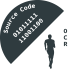
\includegraphics[width=0.5\textwidth]{images/Logo1.pdf}
  \caption{Mein Bild}
\end{figure}

\section{Tabellen}
\begin{table}[h]
  \centering
  \begin{tabular}{c|c}
    Spalte 1 & Spalte 2 \\
    \hline
    Eintrag 1 & Eintrag 2 \\
  \end{tabular}
  \caption{Meine Tabelle}
\end{table}

\section{Mathematik}
\begin{align}
  E &= mc^2
\end{align}

\section{Quellcode}
\begin{lstlisting}[language=Python]
print("Hallo Welt!")
\end{lstlisting}

\section{Literaturverzeichnis}
Ein interessantes Papier ist das von \textcite{beispiel}.

\end{document}
